\documentclass[../3Wworkreport.tex]{subfiles}
\doublespacing

\begin{document}

\chapter{Analysis}
\label{chap:analysis}

To capitalize on the ideas provided by quantum mechanics, one can associate $x$ with the $d$-dimensional qudit $\ket{\psi}$, where in the measurement basis, denoted $\set{\ket{j}}_{j=0}^{d-1}$, $\ket{\psi}= x$. By considering the vector $x$ as the mathematical representation of the quantum state $\ket{\psi}$, some of the tools provided by the discrete Wigner function become useful in solving this problem. By adapting the protocol outlined in \cite{Pashayan2014} for each problem, one can arise at some classical computational protocols that solve Raz's problem probabilistically.\\
%The two solutions are more technical in nature, and are given in \autoref{app:protocol1} and \autoref{app:protocol2}. It is highly recommended the reader review these appendices in order to follow the complexity analysis in the following subsections.

A key point to note is that throughout both of these protocols, no quantum computation ever occurs. These solutions are inspired by the stabilizer sub-theory, which behaves differently than general quantum computation. Additionally, calculating $\hat{x}$ between Step 5 and Step 6 in Protocol 1 (and similarly calculating $\hat{v}$ between Step 6 to Step 7 in Protocol 2) can be done since the vectors $x$ and $Ux$ are real (and thus $\ket{\psi}$ and $U\ket{\psi}$ are as well). If one was to perform a basis measurement on $\ket{\psi}$ and $O$ is the random variable associated with the measurement outcome, then $O$ is associated with the distribution Pr$(O = k) = |\braket{\psi|k}|^2$. The value of the probability is the square of the $k$th component of $\ket{\psi}$. Computing the sample probability Pr($O = k$) approximates the value of the $k$th element of $x$ in Protocol 1. Doing this for each $k$ produces the values of the vector $\hat{x}$. The same idea holds for $U\ket{\psi}$ and the $k$th value of $Ux$ in Protocol 2, using Pr$(O = k) = |\Braket{\psi |U|k}|^2$.

\section{Protocol 1: Solution to Problem 1}
\label{sec:protocol1}
\begin{enumerate}
	\item
		Let $\rho = \ket{\psi}\bra{\psi}$, and let $W_\rho$ and $\mathcal{M}_\rho$ be as defined in \autoref{app:dwf}.
	\item
		Alice samples a value $\alpha \in \mathbb{Z}_d^2$ according to the weighted probability distribution 
		\begin{equation}
			\text{Pr}(\alpha) = \frac{|W_\rho(\alpha)|}{\mathcal{M}_\rho}
		\end{equation}
		and sends $\alpha$ to Bob. She also sends Sgn($W_\rho(\alpha)$) and $\mathcal{M}_\rho$ (some positive real number). Alice will need to send back a truncated value of $\mathcal{M}_\rho$, denoted $\hat{\mathcal{M}}_\rho$, since sending the entire real number can in principle use an infinite amount of information. How precise this truncated value needs to be will be discussed in \autoref{sec:complexity}.

	\item
		Bob samples possible measurement outcomes from the distribution
		\begin{equation}
			\text{Pr}(O = k | \alpha) = |W_{E_k}(\alpha)|
		\end{equation}

	\item
		Bob sets the value
		\begin{equation}
			r = \hat{\mathcal{M}}_\rho W_{E_k}(\alpha) \text{Sgn}(W_\rho(\alpha))
		\end{equation}
		He can regard this value as a realization of some random variable $R$, whose probability distribution is given by
		\begin{equation}
			\text{Pr}(R = r) = \frac{|W_\rho(\alpha)|}{\mathcal{M}_\rho}
		\end{equation}

	\item
		Alice and Bob repeat steps 2-4 $T_1$ times, and Bob calculates $\hat{R}$, the sample average of $R$ over the $T_1$ repetitions. The particular value for $T_1$ is another topic of interest, and is discussed in \autoref{sec:convergence_repetitions}. As shown in \cite{Pashayan2014},
		\begin{equation}
			\mathbb{E}(R) = \text{Pr}(E_k| \rho)
		\end{equation}
		where $\mathbb{E}(R)$ is the expected value of $R$. By doing this, Bob can approximate the measurement probabilities and create an estimate, $\hat{x}$, for the vector $x$.

	\item
		On his computer, since Bob has the vector $\hat{x}$, he computes d($\hat{x}, M_0)$, which does not require any further communication, and outputs 1 or 0, depending on the result.
\end{enumerate}

\section{Protocol 2: Solution to Problem 2}
\label{sec:protocol2}
\begin{enumerate}
	\item
		Let $\rho = \ket{\psi}\bra{\psi}$, and let $W_\rho$ and $\mathcal{M}_\rho$ be as defined in \autoref{app:dwf}.
	\item
		Alice samples a value $\alpha \in \mathbb{Z}_d^2$ according to the weighted probability distribution 
		\begin{equation}
			\text{Pr}(\alpha) = \frac{|W_\rho(\alpha)|}{\mathcal{M}_\rho}
		\end{equation}
		and sends $\alpha$ to Bob.

	\item
		Bob has the orthogonal (which is, by definition, unitary) matrix $U$, so by using the Wigner representation of $U$, $W_U$, he now samples $\beta \in \mathbb{Z}_d^2$ according to the distribution
		\begin{equation}
			\text{Pr}(\beta|\alpha) = \frac{|W_U(\beta|\alpha)|}{\mathcal{M}_U(\alpha)}
		\end{equation}
		Bob sends $\beta$ to Alice, along with Sgn($W_U(\beta|\alpha)$) and $\hat{\mathcal{M}}_U(\alpha)$. Like in the previous protocol, the precision to which Bob can send back $\hat{\mathcal{M}}_U(\alpha)$ needs to be specified. This will also be discussed in \autoref{sec:complexity}.

	\item
		Alice samples possible measurement outcomes from the distribution
		\begin{equation}
			\text{Pr}(O = k | \beta) = |W_{E_k}(\beta)|
		\end{equation}

	 \item
		Alice sets the value
		\begin{equation}
			r = \hat{\mathcal{M}}_U(\alpha) \mathcal{M}_\rho W_{E_k}(\beta) \text{Sgn}(W_\rho(\alpha) W_U(\beta|\alpha))
		\end{equation}
		Alice regards this value as a realization of some random variable $R$, whose probability distribution is given by
		\begin{equation}
			\text{Pr}(R = r) = \frac{|W_\rho(\alpha)|}{\mathcal{M}_\rho} \frac{|W_U(\beta|\alpha)|}{\mathcal{M}_U(\alpha)}
		\end{equation}

	\item
		Alice and Bob repeat steps 2-5 $T_2$ times, and Alice calculates $\hat{R}$, the sample average of $R$ over the $T_2$ repetitions (this value will also be discussed in \autoref{sec:convergence_repetitions}). As shown in \cite{Pashayan2014},
		\begin{equation}
			\mathbb{E}(R) = \text{Pr}(E_k| \rho, U)
		\end{equation}
		By doing this, Alice can approximate the measurement probabilities and create an estimate, $\hat{v}$, for the vector $Ux$.

	\item
		Alice computes d($\hat{v}, M_0)$, which does not require any communication, and outputs 1 or 0, depending on the result. 
\end{enumerate}

\section{Convergence and Repetition of the Protocols}
\label{sec:convergence_repetitions}
The sample average, $\hat{R}$, over $T$ repetitions obeys the Chernoff-Hoeffding inequality, as explained in \cite{Pashayan2014}.
\begin{alignat}{1} \label{eq:chernoff}
	\text{Pr}(|\hat{R} - \mathbb{E}(R)|) \ge \epsilon) \le 2e^{\frac{-T\epsilon^2}{2\mathcal{M}^2}}
\end{alignat}
where $\mathcal{M} = \mathcal{M}_\rho\mathcal{M}_U$, the total mana of the system (refer to \autoref{app:dwf} for more information). Thus, if $T$ is large enough for each solution, then probabilistic convergence is guaranteed. In order to determine $T$, finding an upper bound for $\mathcal{M}$ is required. This value of $\mathcal{M}$ depends on $x$ and the matrix $U$, but some upper bound for $\mathcal{M}$ can be established. The next few subsections are dedicated to characterizing special cases of $\mathcal{M}$ given certain types of $U$ and $x$.

\subsection{Mana of General States and Matrices}
\label{subsec:cr_general}
Bounding $\mathcal{M}$ in a general case can be done by using the following propositions. Their proofs are listed in \autoref{app:proofs} for reference.
\begin{prop}\label{prop:manarho}
	For any quantum state $\rho, \mathcal{M}_\rho \le \sqrt{d}$.
\end{prop}
\begin{prop}\label{prop:manaunitary}
	For any unitary (and by definition, orthogonal) matrix $U, \mathcal{M}_U \le d$.
\end{prop}
This information states that for Protocol 1, $\mathcal{M} = \mathcal{M}_\rho \le \sqrt{d}$, so \autoref{eq:chernoff} becomes
\begin{equation}
	\text{Pr}(|\hat{R} - \mathbb{E}(R)|) \ge \epsilon) \le 2e^{\frac{-T_1\epsilon^2}{2d}}
\end{equation}
This convergence becomes independent of the dimension $d$ if $T_1 = d$, which is a desirable quality of an algorithm. Similarly for Protocol 2, $\mathcal{M} = \mathcal{M}_U \mathcal{M}_\rho \le d\sqrt{d}$, and thus setting $T_2 = d^{3/2}$ will remove the dependence of the size of $x$ from the convergence of the protocol.

\subsection{Mana of Stabilizer States and Clifford Gates}
\label{subsec:cr_stabilizer}
As is discussed in \autoref{app:dwf}, the discrete Wigner function and the stabilizer sub-theory are intimately connected, so using an algorithm based on the discrete Wigner function will likely behave in special ways when dealing with stabilizer states and unitary matrices. The following propositions are useful for characterizing the stabilizers in these solutions:
\begin{prop}
	For any stabilizer state $\ket{\phi}$, $W_{\ket{\phi}\bra{\phi}}(\alpha) \ge 0$.
	\label{prop:wignerstabilizer}
\end{prop}
\begin{prop}
	For any Clifford unitary $U$, $W_U(\beta|\alpha) \ge 0$.
	\label{prop:wignerclifford}
\end{prop}
\autoref{prop:wignerstabilizer} is also known as Hudson's Theorem for finite-dimensional quantum systems, and the proof of both of these propositions is given by Daniel Gross \cite{Gross2006}. The positive nature of the Wigner function for stabilizer states and Clifford gates yields the following corollaries.
\begin{corol}
	For any stabilizer state $\ket{\phi}$, $\mathcal{M}_{\ket{\phi}\bra{\phi}} = 1$.
	\label{corol:manastab}
\end{corol}
\begin{corol}
	For any Clifford unitary, $U$, $\mathcal{M}_U(\alpha) = 1$ for all $\alpha \in \mathbb{Z}_d^2$.
	\label{corol:manaclif}
\end{corol}
These follow immediately from the above propositions and the properties of the discrete Wigner function given in \autoref{app:dwf}. This means that the in the case of states and matrices guaranteed to be in the stabilizer sub-theory, calculating the mana is unnecessary, and the concerns raised in Step 2 of Protocol 1 and Step 3 of Protocol 2 can be ignored. Better yet, due to the positive properties of stabilizers, Alice and Bob can use a geometric argument to produce an efficient protocol. As stated in \autoref{app:dwf}, stabilizer states form lines in the discrete phase space. Lines in this space are specified by $ax + bz = p$ (mod $d)$, and an individual line can be uniquely determined by two points if $d$ is prime.\\ \\

\begin{figure}[h]
	\begin{center}
		\subfloat[An eigenstate of $Z$]{\label{fig:stabps_a}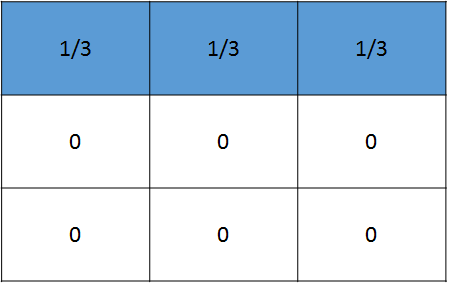
\includegraphics[width=0.4\textwidth]{Z_stab_dps.png}}
		\subfloat[An eigenstate of $\omega^{-2^{-1}}ZX$]{\label{fig:stabps_b}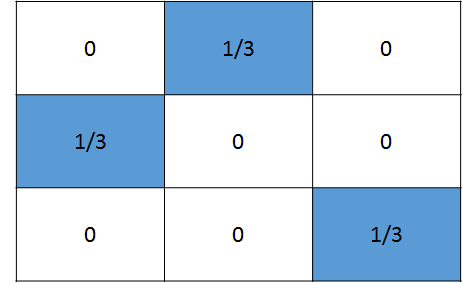
\includegraphics[width=0.4\textwidth]{XZ_stab_dps.png}}\\
		\subfloat[A typical non-stabilizer state]{\label{fig:stabps_c}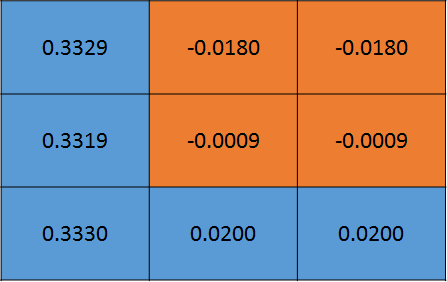
\includegraphics[width=0.4\textwidth]{rand_dps.png}}
		\caption[Discrete phase space and stabilizer states]{The stabilizer states form a line in the discrete phase space ($d = 3$ shown), while non-stabilizer states do not.}
	\end{center}
\end{figure}

Alice can specify what state $x$ is by sending Bob four integers (two points in the discrete phase space that have non-zero values) since that specifies a line. Bob then knows exactly what state Alice has. Using \autoref{fig:stabps_a} for example, Alice could send (0,0) and (0,1) to Bob (the northwest and noth points in the grid), and he would know for certain which eigenstate of the $Z$ matrix $x$ was. In Problem 2, since Clifford matrices map stabilizer states to stabilizer states, $Ux$ will form a line in the phase space, and Bob can send four integers back to Alice that specify two non-zero elements. Working in the stabilizer sub-theory ensures a simple and effective way of solving both Problem 1 and Problem 2.

\section{Communication Complexity of the Protocols}
\label{sec:complexity}
Without considering the precision on the mana values, \autoref{tab:step_complex} shows the maximum communication complexity of each step in Protocols 1 and 2. The communication complexity behaves like $O(T_1$ log $d)$ for Protocol 1 and $O(T_2$ log $d)$ for Protocol 2. Given the analysis of repetitions required for each protocol in \autoref{sec:convergence_repetitions}, the complexities for each problem can be stated concisely. This is done in \autoref{tab:protocol_complex}.\\

\begin{table}[h]
\begin{center}
\begin{tabular}{r | c | c}
	\textbf{Step No.} & \textbf{Protocol 1} & \textbf{Protocol 2}\\\hline
	Step 1 & 0 bits & 0 bits \\\hline
	Step 2 & 2 log$d$ bits & 2 log$d$ bits \\\hline
	Step 3 & 0 bits& 2 log$d$ bits \\\hline
	Step 4 & 0 bits & 0 bits\\\hline
	Step 5 & $T_1$ times & 0 bits \\\hline
	Step 6 & 0 bits & $T_2$ times\\\hline
	Step 7 & N/A & 0 bits \\\hline
\end{tabular}
\end{center}
	\caption{Communication complexity of each step in the two protocols.}
	\label{tab:step_complex}
\end{table}

\begin{table}[h]
\begin{center}
\begin{tabular}{l | p{0.14\textwidth} | p{0.13\textwidth} | p{0.14\textwidth} | p{0.13\textwidth}}
	& {\bfseries Stabilizer $x$, Clifford $U$}
		& \textbf{General $x$, Clifford $U$}
		& \textbf{Stabilizer $x$, General $U$}
		& \textbf{General $x$, General $U$}\\\hline
	\textbf{Problem 1}
		& $\bullet$ $O($log $d)$\newline $\bullet$ 1 round\newline $\bullet$ one-way
		& $\bullet$ $O(d$ log $d)$\newline $\bullet$ $d$ rounds\newline $\bullet$ one-way
		& N/A
		& N/A \\\hline
	\textbf{Problem 2}
		& $\bullet$ $O($log $d)$\newline $\bullet$ 1 round\newline $\bullet$ two-way
		& $\bullet$ $O(d$ log $d)$\newline $\bullet$ $d$ rounds\newline $\bullet$ two-way
		& $\bullet$ $O(d^2$ log $d)$\newline $\bullet$ $d^2$ rounds\newline $\bullet$ two-way
		& $\bullet$ $O(d^3$ log $d)$\newline $\bullet$ $d^3$ rounds\newline $\bullet$ two-way \\\hline
\end{tabular}
\end{center}
	\caption[Communication complexity of protocols.]{Communication complexity, number of rounds, and what type of communication (one-way or two-way) for each protocol in specified input cases.}
	\label{tab:protocol_complex}
\end{table}

In order to keep the complexities listed, $\hat{\mathcal{M}}_U(\alpha)$ and $\hat{\mathcal{M}}_\rho$ must be transmitted in $O($log $d)$ bits, or less, for each case. For unsigned real numbers (unsigned numbers can be used since the mana is always positive), this can be done using the Institute of Electrical and Electronics Engineers (IEEE) convention, since the mana is always bounded by $d$. For example, if a number is expressed as $a = c2^q, c,q \in \mathbb{Z}$, letting $c$ be 3 log $d$ digits long (log $d$ digits ensures it can reach the value $d$, and the other 2 log $d$ can be for extra precision in the numbers to the right of the decimal) and $q \in [0, 2$ log $d]$ will ensure the decimal point can reach where it needs to be. Sending these two integers $c$ and $q$ can be expressed in $O($log $d)$ bits, which is the desired result. Thus, Alice and Bob can communicate these mana values while achieving high precision and not changing the overall communication complexity of the protocols.

\end{document}